\chapter{Disseny e implementaci\'{o}}
\label{cha:dessign}

En aquest cap\'{i}tol veurem els patrons de dissenys emprats i les tecnologies implementades. Tamb\'{e} descriurem la interf\'{i}cie d'usuari m\'{e}s complexa i el fluxe de les operacions de sistema


\section{Esquema general arquitect\'{o}nic del sistema}
A continuaci\'{o} veiem un gr\`{a}fic amb els principals components del sistema i com es relacionen.

\begin{figure}[h]
  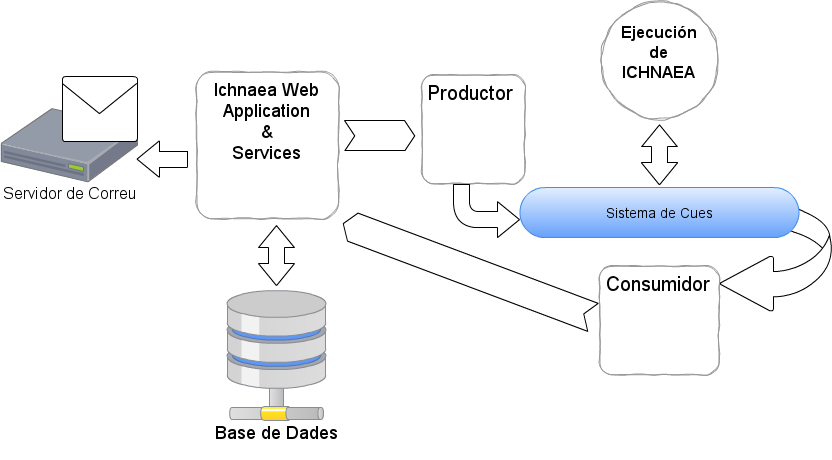
\includegraphics[scale=0.5]{img/design/ArchitectureSoftware.png}
  \caption{Arquitectura del sistema}
  \label{dessign:archsoftware}
\end{figure}
On:
\begin{itemize}
\item Ichnaea Web Application & Services \'{e}s el codi de la aplicaci\'{o} i els serveis HTTP
\item Servidor de correu \'{e}s el servidor SMTP per enviar correus electr\`{o}nics als usuaris
\item Productor-Cua-Consumidor \'{e}s el sistema de cues. Expliquem el paradigma a cap\'{i}tol \ref{dessign:queue_system_overview}. La funci\'{o} \'{e}s gestionar els inicis, fluxes i finals d'execucions de Ichnaea.
\item La base de dades on es guardan els contiguts i models de dades i resultats.
\end{itemize}

\section{Patr\'{o} de disseny}
Per la implementaci\`{o} del sistema web s'han usat un disseny per capes(Presentaci\'{o}, domini i persistencia de dades) amb els seg\�{u}ents patrons de disseny:
  \begin{itemize}
  \item Model-Vista-Controlador amb controlador frontal
  \item Capa de Servei
  \item Injecci\'{o} de depend\`{e}ncies
  \item Repositori de model de dades
  \item Capa de mapejat de dades
  \item View template
  \item Interficies enriquides amb servei webs
  \end{itemize}

\subsection{Esquema del disseny}
\begin{figure}[h]
  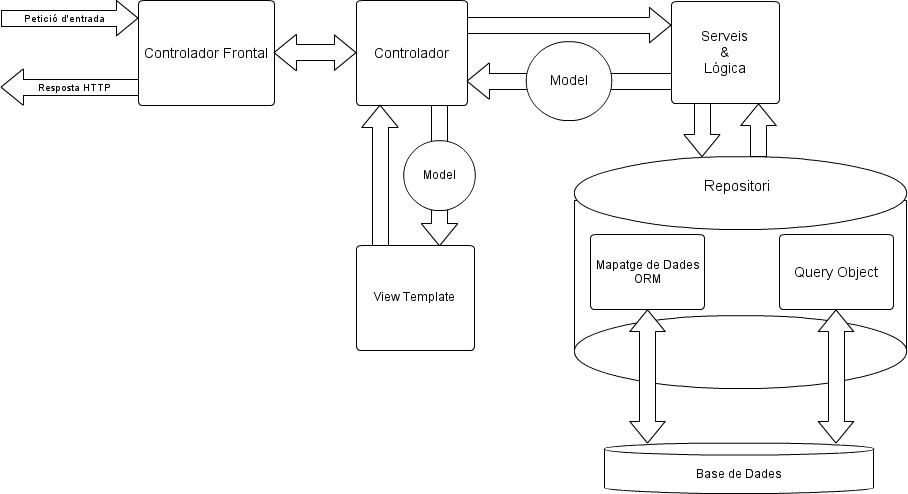
\includegraphics[scale=0.4]{img/design/IchnaeaPatterns.png}
  \caption{Patrons de disseny}
  \label{dessign:dessignpatters}
\end{figure}

Els components MVC,Model-Vista-Controlador, amb controlador frontal \'{e}s un disseny t\'{i}pic en les aplicacions web on:
\begin{itemize}
\item el model \'{e}s una representaci\'{o} de les dades en les que treballa la aplicaci\'{o}
\item la vista transforma el model a un format visible i llegible
\item el controlador frontal rep totes les peticions i les redirigeixs als controladors corresponents
\item el controlador se encarrega de processar les peticcions especifiques
\end{itemize}
L'arquitectura MVC separa la capa de presentaci\'{o} de la l\`{o}gica de domini. La capa de presentaci\'{o} accedeix a la capa de domini mitjan�ant serveis, injectant depend\'{e}ncies. \\
La injecci\'{o} de depend\'{e}ncies \'{e}s un patr\'{o} a on es suministren objectes a una clase en lloc de ser la clase qui crea els objectes\cite{dependency_injection}. Les avantatges de usuar DI(''dependency injection''):
\begin{itemize}
\item Codi m\'{e}s f\`{a}cil de mantenir, extendre o modificar
\item Desenvolupament guiat per proves (Test Driven Development o TDD en angl\'{e}s)
\item DI ens obliga a planejar una mica millor les nostres depend\`{e}ncies; decidim si una clase realment necesita d'un altre objecte per realitzar la seva funci�.
\end{itemize}
Els serveis, en aquest cas, contenen l\'{o}gica de Ichnaea. Accedeixen mitjan�ant les dades repositoris d'objectes. Els repositoris son mediadors entre el domini i les dades pesistents. Els repositoris retornen entitats de la l\'{ogica}. El mapatge de dades ORM(''Object Relational Mapping''), mapatge objecte-relacional, \'{e}s un patr\'{o} de disseny, encara que alguns enginyers els agrada dir que \'{e}s una tecnica de programaci\'{o} i a uns altres una tecnologia, que estableix una relaci\'{o} directe entre les entitats i la dades persistents.\cite{orm}

\section{Implementaci\'{o} i tecnologies}
\subsection{Symfony}
Symfony2 \'{e}s un HTTP framework per a PHP. Nativament implementa una variaci\'{o} del Model-Vista-Controlador amb controlador frontal amb injecci\'{o} de depencies a la capa de serveis.\cite{symfony} \\
Arquitectonicament, Symfony2 estructura el codi en Bundle, similar als paquets de JAVA. Els ''bundle'' son un conjunt de serveis, entitats i recursos independents entre si. Els bundles implementats son:
\begin{itemize}
\item{Bundle de usuaris: UserBundle}. Paquet de serveis, vistes i recursos per usuaris. S'ha utilitzat un paquet de Symfony: FOSUserBundle.\cite{fosuserbundle}. S'ha fet una extensi\'{o} del paquet per implementar la gesti\'{o} de rols i grups.
\item{Bundle de matrius: MatrixBundle}. Paquet de serveis, vistes i recursos per les matrius.
\item{Bundle de trainings: TrainingBundle}. Paquet de serveis, vistes i recursos per els entrenaments(''trainings'').
\item{Bundle de serveis webs: ApiBundle}. Paquet de serveis,vistes i recursos per la API JSON Restful. 
\item{Bundle de predicci\'{o}: PredictionBundle}. Paquet de serveis, vistes i recursos per les matrius de prediccions.
\end{itemize}

\subsection{Recursos}
La estructura de recursos de la aplicaci\'{o} \'{e}s la seg\�{u}ent:\\

\begin{tabular}{| l | l |}
\hline
Matrius       & matrix/(id) \\ \hline
''Trainings''  & matrix/(id)/training/(id) \\ \hline
''Predctions'' & matrix/(id)/training/(id)/prediction/(id) \\ \hline
\end{tabular}

S'ha emprat aquesta estructura de recursos degut a les depencies entre les diferentes entitats. Un ''training'' dep\'{e}n d'una matriu i una predicci\'{o} dep\'{e}n d'un ''training''.

\section{Servei web}
S'ha desenvolupat una llibreria API JSON Restful\cite{apijson} per enriquir les interficies. S'ha emprat aquesta tecnologia per la escalabilitat que aporta i perque en un futur es pogui aprofitar el desenvolupament d'aquesta.
Les operacions, els recursos i el parametres son:\\
\begin{tabular}{ | l | l |}
\hline
GET & /api/season/(id) \\ \hline
POST & /api/season/searchByName \\ \hline
     & INPUT: \{'pattern': string\} \\ \hline
     & OUTPUT: ['string-match-1',...,'string-match-n'] \\ \hline
GET & /api/variable/(id)/seasonSet \\ \hline
DELETE & /api/variable/(id)/seasonSet/(id)\\ \hline
DELETE & /api/variable/(id)/seasonSet/(id) /component/(id) \\ \hline
DELETE & /api/variable/(id)/seasonSet/(id) /component/(id)/complete\\ \hline
PUT & /api/matrix/(id)/column/(id)\\ \hline
PUT & /api/matrix/(id)/sample/(id)\\ \hline
\end{tabular}
Les peticions estan seguritzades per ''cookies'' amb l'usuari. 

\section{Integraci\'{o} amb el sistema de cues RabbitMQP}
\subsection{Introducci\'{o} a l'arquitectura de cues: AMQP}
\label{dessign:queue_system_overview}
L'est\`{a}ndard AMQP (''Advanced Message Queuing Protocol'') \'{e}s un protocol d'est\`{a}ndard obert en la capa d'aplicacions d'un sistema de comunicaci�. Les caracter�stiquess que definen al protocol AMQP son la orientaci� a missatges, encuament(''queuing''), enrutament i exactitud, entre altres com,per exemple, la seguretat o les suscripcions.\cite{amqp}\\
AMQP defineix una s\`{e}rie d'entitats. Desde la perspectiva de la interconnexi� les m\'{e}s relevants son:
\begin{itemize}
\item El corredor de missatges: un servidor on els clients AMQP es conecten usant el protocol AMQP. Els corredores de missatges poden executar-se en un entorn distribu\�{i}, pero aquesta capacitat \'{e}s espec\'{i}fica de la implementaci�.
\item Usuari: un usuari \'{e}s una entitat amb credencial pot ser autoritzat a conectar-se a un corredor.
\item Connexi�: una connexi\'{o} f\'{i}sica, usant per exemple TCP/IP, entre el corredor i l'usuari.
\item Clients: productors i consumidors. EXPLICAR PRODUCTORS I CONSUMIDORS.
\end{itemize}

RabbitMQ \'{e}s un software que implementa aquest protocol. El sistema de cues est\'{a} implementat per Miguel Ibero. I ofereix una ofereix una llibreria per la seva integraci\'{o}. 

\subsection{Consumidors i gesti\'{o} de resultats}
Les respostes de les execucions de Ichnaea enviades per la cua (mirar la figura \ref{dessign:archsoftware}), les rep el consumidor. \\
Symfony2 permet crear comandes CLI per crear processos. Els consumidors necessiten ser processos ''stand-alone''(aut\'{o}noms) que escoltin les sortides, consumeixin, els resultats de la cua. \\
L'esquelet d'una comanda per aquests consumidors actualment \'{e}s:
\begin{lstlisting}
class ConsumerCommand extends ContainerAwareCommand
{
	//Definicio de la comanda
	protected function configure()
	{
		$this
		->setName('nom_de_la_comanda')
		->setDescription('Consumer server');
	}
	
	//Execucio de la comanda
	protected function execute(InputInterface $input, OutputInterface $output)
	{
		//Interficie per integrar el sistema de cues
		$amqp = new AmqpConnection('URI_per_fer_la_connexio');
		$amqp->open();
		
		//Crida al servei
		$servei = $this->getContainer()->get('nom_de_servei');
		
		//Crear el consumidor, amb una 
		//funcio que es crida quan la 
		//cua estableix comunicacio amb 
		//un objecte de la resposta esperada 
		//i li passa el servei 
		$amqp->listenForBuildModelResponse(function (ObjectResponse $resposta_de_la_cua) use ($servei){
			$servei->actualitzaDades($resposta_de_la_cua);
		});
		$amqp->wait();
	}
}
\end{lstlisting}

\subsubsection{Consumidor ''trainings''}
El consumidor de ''trainings'' es queda escoltant les respostes del servei de \\

\section{Interf\'{i}cies}
Les interf\'{i}cies s'ha dissenyat enriquides i 
\subsection{Interf\'{i}cie de configuraci\'{o} de matrius}
\subsection{Interficies de carrega de matrius per fitxers }
Per carregar les matrius s'ha emprat les noves funcionalitats HTML5 per llegir fitxers desde els propis clients web(navegadors). La selecci\'{o} de fitxers s'ha utilitzat la etiqueta <file> i els events BLAH BLAH. En una variable deshabilitada(en properes versions hauria de ser oculta) es carrega el contingut del fitxer.





